\documentclass[11pt, a4paper]{article}
\usepackage{pdfpages}
\usepackage{parallel}
\usepackage[T2A]{fontenc}
%\usepackage{ucs}
\usepackage[utf8]{inputenc}
\usepackage[english,russian]{babel}
\usepackage{hyperref}
\usepackage{rotating}
\usepackage[inner=2cm,top=1.8cm,outer=2cm,bottom=2.3cm,nohead]{geometry}
%\usepackage{listings}
\usepackage{graphicx}
\usepackage{wrapfig}
\usepackage{longtable}
\usepackage{indentfirst}
\usepackage{array}
\usepackage{tikzsymbols}
\usepackage{soul}
\usepackage[ruled,vlined]{algorithm2e}
\usepackage{qrcode}
\counterwithout{figure}{section} 

\usepackage{url}
\makeatletter
\g@addto@macro{\UrlBreaks}{\UrlOrds}
\makeatother

\newcolumntype{P}[1]{>{\raggedright\arraybackslash}p{#1}}
\frenchspacing
%\usepackage{fixltx2e} %text sub- and superscripts
\usepackage{icomma} % коскі ў матэматычным рэжыме
%\PreloadUnicodePage{4}

\newcommand{\longpage}{\enlargethispage{\baselineskip}}
\newcommand{\shortpage}{\enlargethispage{-\baselineskip}}

\def\switchlang#1{\expandafter\csname switchlang#1\endcsname}
\def\switchlangbe{
\let\saverefname=\refname%
\def\refname{Літаратура}%
\def\figurename{Іл.}%
}
\def\switchlangru{
\let\saverefname=\refname%
\let\savefigurename=\figurename%
\def\refname{Литература}%
\def\figurename{Рис.}%
}
\def\switchlangen{
\let\saverefname=\refname%
\def\refname{References}%
\def\figurename{Fig.}%
}

\hyphenation{admi-ni-stra-tive}
\hyphenation{ex-pe-ri-ence}
\hyphenation{fle-xi-bi-li-ty}
\hyphenation{Py-thon}
\hyphenation{ma-the-ma-ti-cal}
\hyphenation{re-ported}
\hyphenation{imp-le-menta-tions}
\hyphenation{pro-vides}
\hyphenation{en-gi-neering}
\hyphenation{com-pa-ti-bi-li-ty}
\hyphenation{im-pos-sible}
\hyphenation{desk-top}
\hyphenation{elec-tro-nic}
\hyphenation{com-pa-ny}
\hyphenation{de-ve-lop-ment}
\hyphenation{de-ve-loping}
\hyphenation{de-ve-lop}
\hyphenation{da-ta-ba-se}
\hyphenation{plat-forms}
\hyphenation{or-ga-ni-za-tion}
\hyphenation{pro-gramming}
\hyphenation{in-stru-ments}
\hyphenation{Li-nux}
\hyphenation{sour-ce}
\hyphenation{en-vi-ron-ment}
\hyphenation{Te-le-pathy}
\hyphenation{Li-nux-ov-ka}
\hyphenation{Open-BSD}
\hyphenation{Free-BSD}
\hyphenation{men-ti-on-ed}
\hyphenation{app-li-ca-tion}

\def\progref!#1!{\texttt{#1}}
\renewcommand{\arraystretch}{2} %Іначай формулы ў матрыцы зліпаюцца з лініямі
\usepackage{array}

\def\interview #1 (#2), #3, #4, #5\par{

\section[#1, #3, #4]{#1 -- #3, #4}
\def\qname{LVEE}
\def\aname{#1}
\def\q ##1\par{{\noindent \bf \qname: ##1 }\par}
\def\a{{\noindent \bf \aname: } \def\qname{L}\def\aname{#2}}
}

\def\interview* #1 (#2), #3, #4, #5\par{

\section*{#1\\{\small\rm #3, #4. #5}}
\ifx\ParallelWhichBox\undefined%
    \addcontentsline{toc}{section}{#1, #3, #4}%
\else%
\ifnum\ParallelWhichBox=0%
    \addcontentsline{toc}{section}{#1, #3, #4}%
\fi\fi%

\def\qname{LVEE}
\def\aname{#1}
\def\q ##1\par{{\noindent \bf \qname: ##1 }\par}
\def\a{{\noindent \bf \aname: } \def\qname{L}\def\aname{#2}}
}

\newcommand{\interviewfooter}[1]{
\vskip 1em
\noindent \textit{#1}
}

\AtEndDocument{\vfill\centering \qrcode{https://github.com/fiowro/mouses/blob/main/\jobname.pdf}}

\switchlang{ru}
\begin{document}

\title{1978 "--- DEC H3060 joystick}
\date{}
\maketitle
\selectlanguage{russian}

Джойстик DEC H3060 (рис. \ref{fig:DecJoystickPic}) был разработан для семейства 16-разрядных миникомпьютеров PDP–11, созданных Digital Equipment Corporation (DEC) в 1970-х годах и продававшихся около 3 десятилетий --- тех самых, для которых изначально создавалась операционная система UNIX. В частности, джойстик чаще всего можно найти в составе видеографической системы VSV11/VS11, которая включала модуль управления курсором/синхронизации нескольких дисплеев, работающий с ним, а также модули видео-памяти и процессора дисплея. Графическое разрешение в различных конфигурациях составляло либо 512x512, либо 512x256 пикселей, 2 или 4 бита на пиксель, с динамическими графическими возможностями, присутствующими в минимальных и отсутствующими в максимальных конфигурациях \cite{joystick}.

Первые упоминания об этом джойстике можно найти в \cite{fiche}, опубликованном в 1978 году, в то время как большая часть источников, ссылающихся на него и VSV11/VS11, появляются начиная с 1981 года \cite{flyer, vsv11}.

\begin{figure}[h]
   \centering
    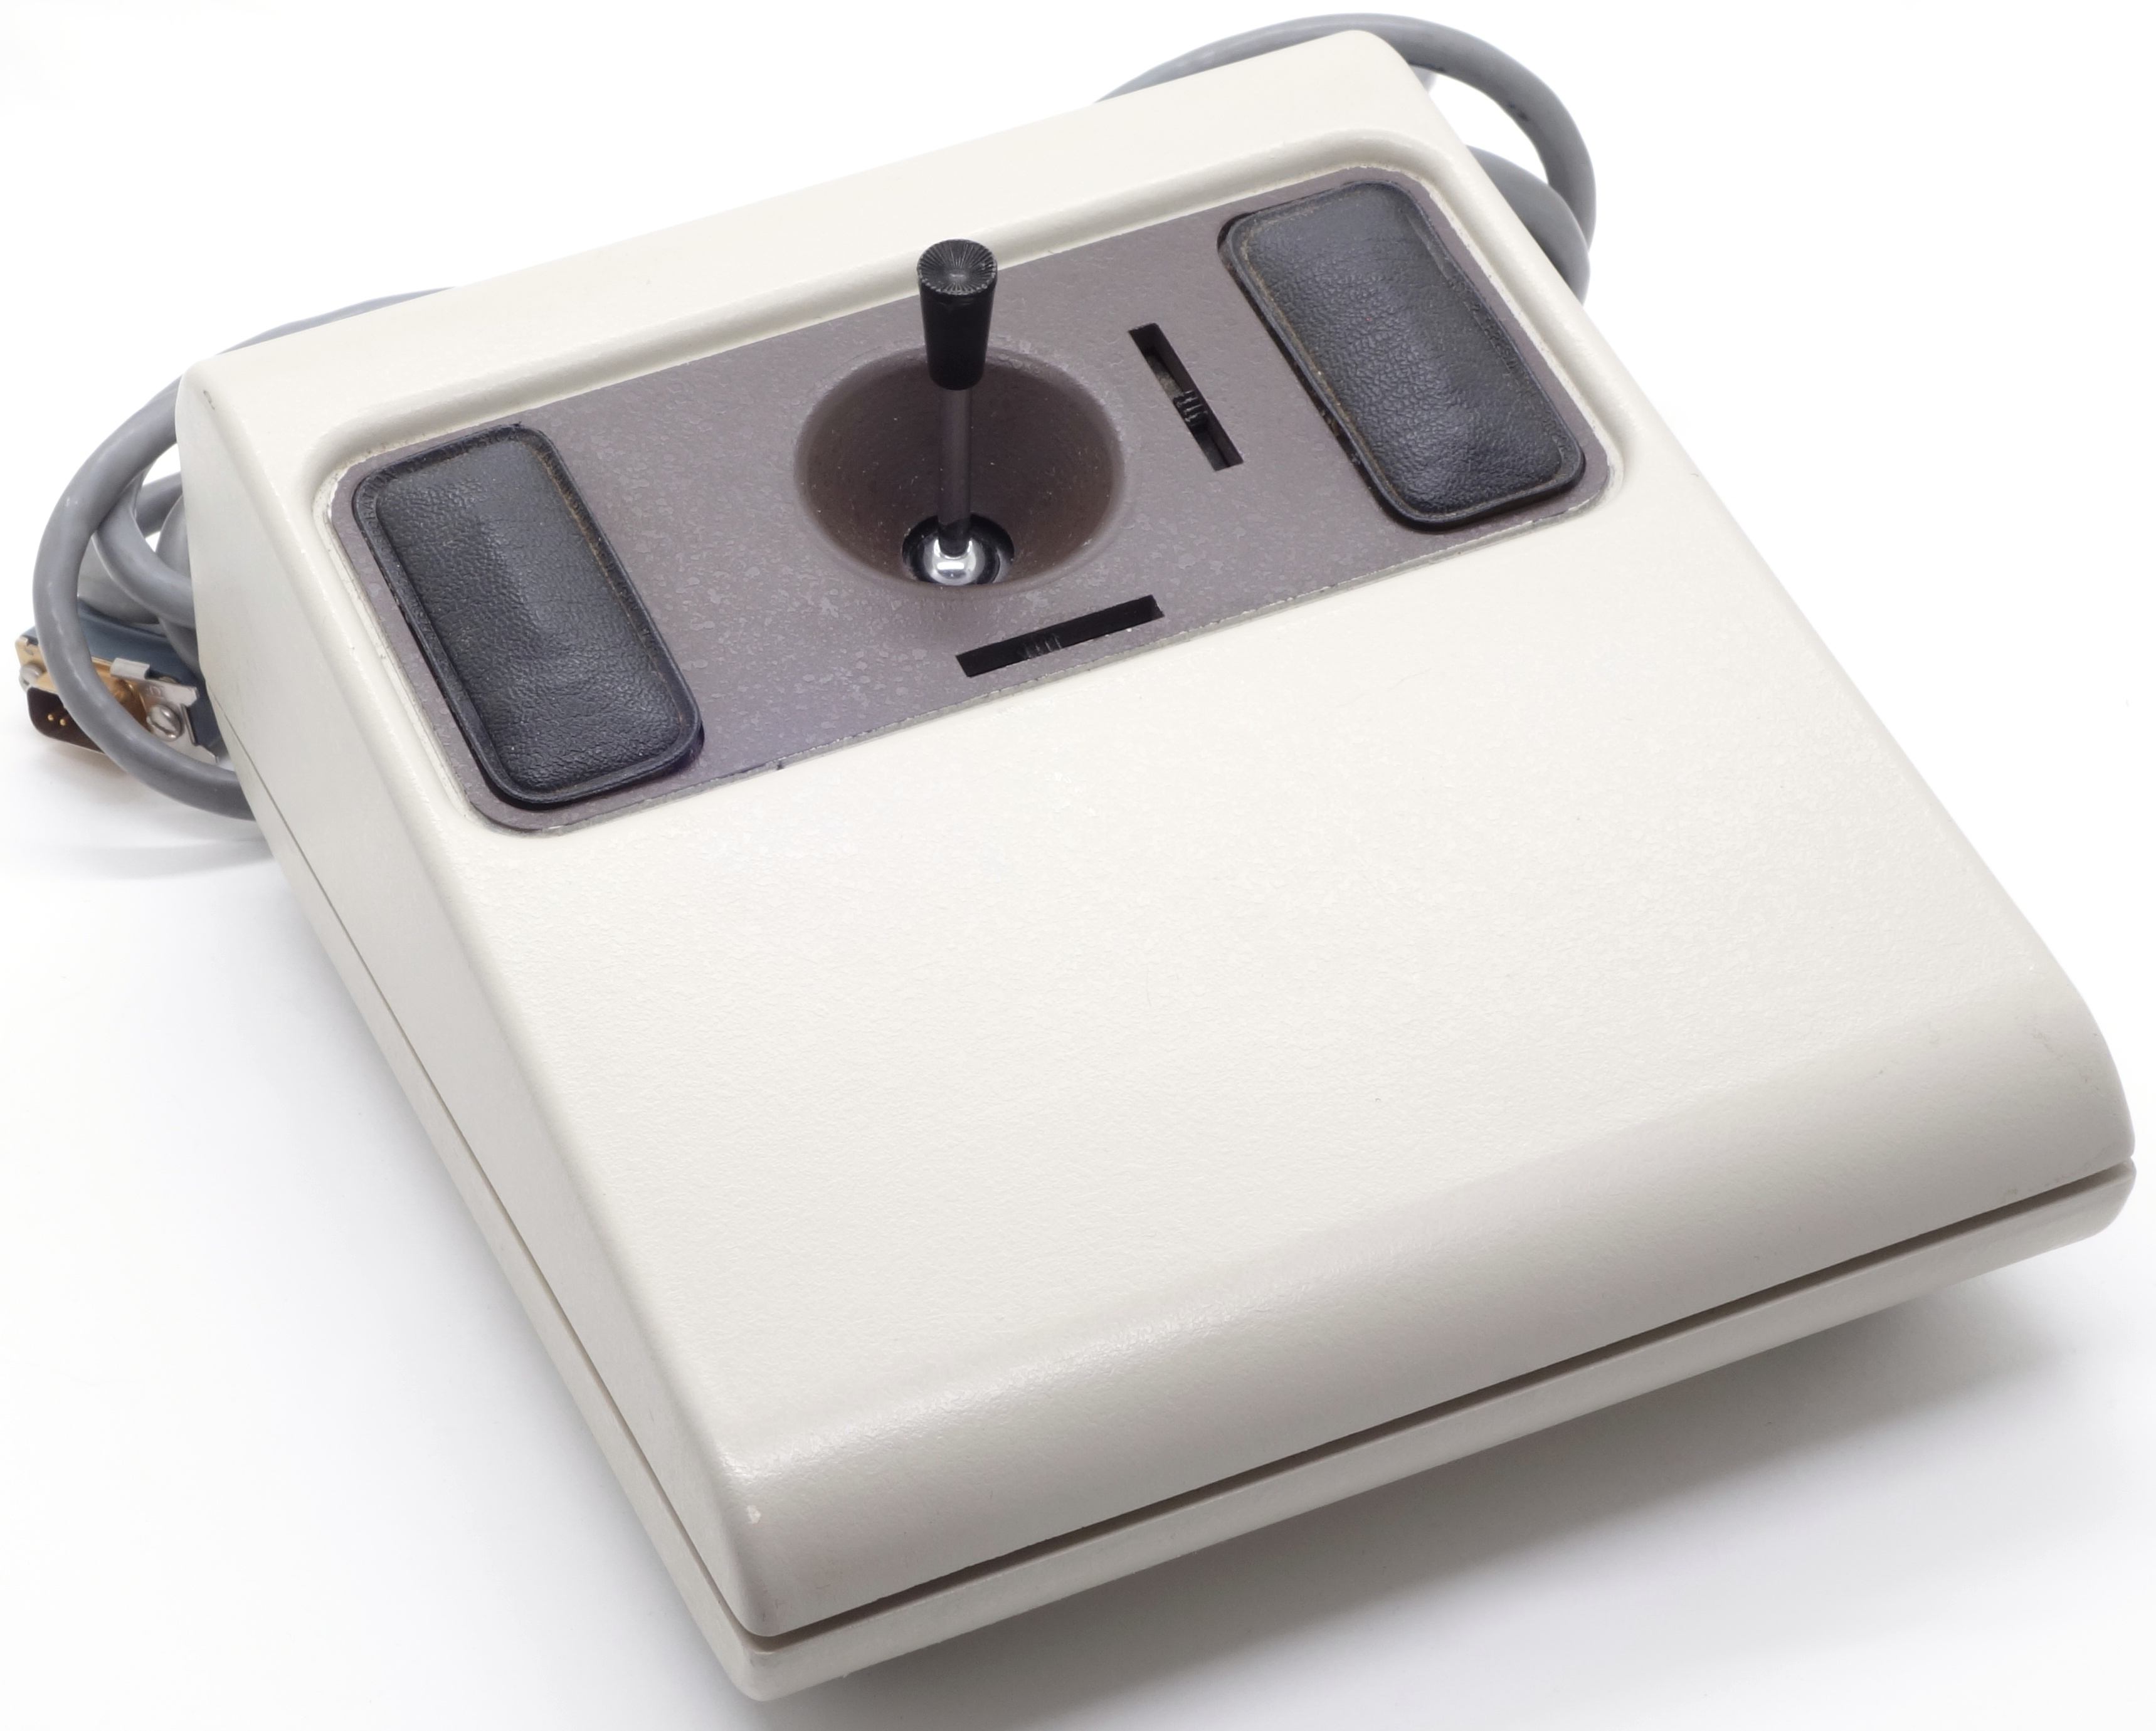
\includegraphics[scale=0.53]{1978_dec_h3060_joystick/pic_30.jpg}
    \caption{Джойстик DEC H3060}
    \label{fig:DecJoystickPic}
\end{figure}

Джойстик имеет резиновые ножки и корпус из бежевого пластика. На верхней стороне (рис. \ref{fig:DecJoystickTopAndBottom}) находится металлическая пластина, объединяющая органы управления: небольшую рукоятку («рычаг», т.~е. «lever» в терминологии производителя), пару кнопок по бокам от нее и два триммера. Кнопки названы производителем <<переключателями прерываний джойстика>> \cite{vsv11} и имеют необычное исполнение в виде дуги из жесткой металлической проволоки с кожаной накладкой \cite{joystick}.

\begin{figure}[h]
    \centering
    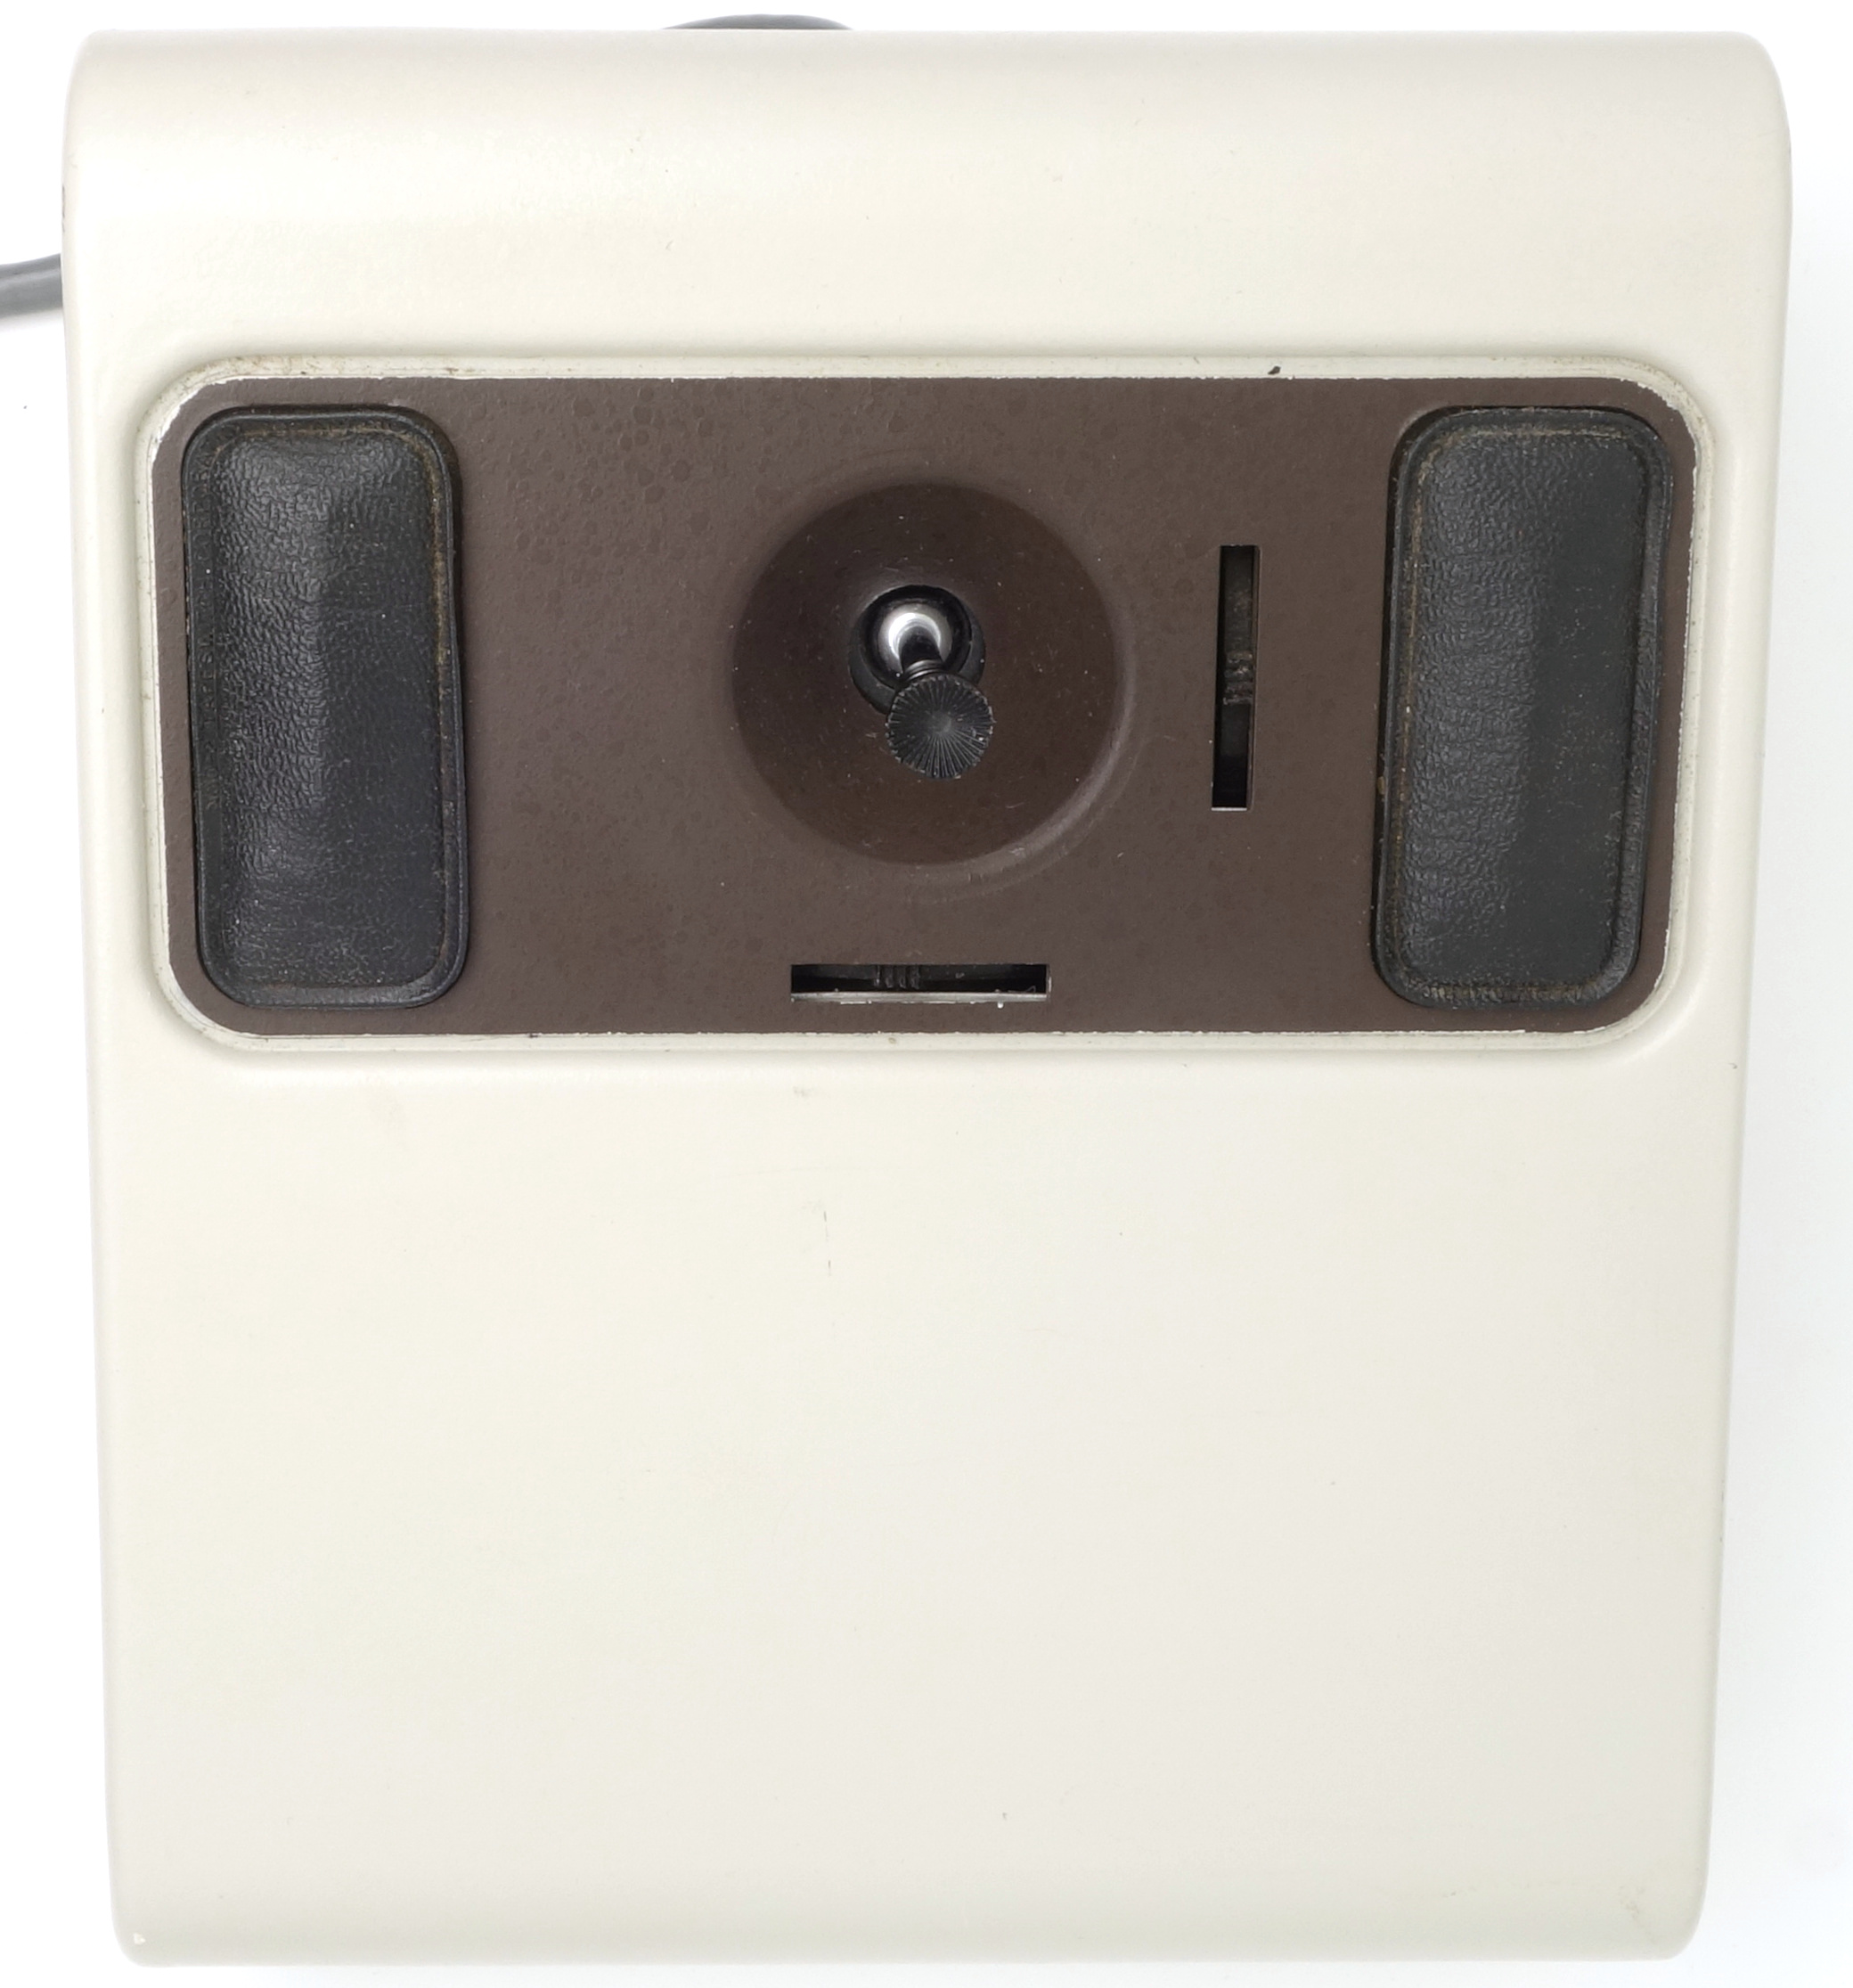
\includegraphics[scale=0.38]{1978_dec_h3060_joystick/top_15.jpg}
    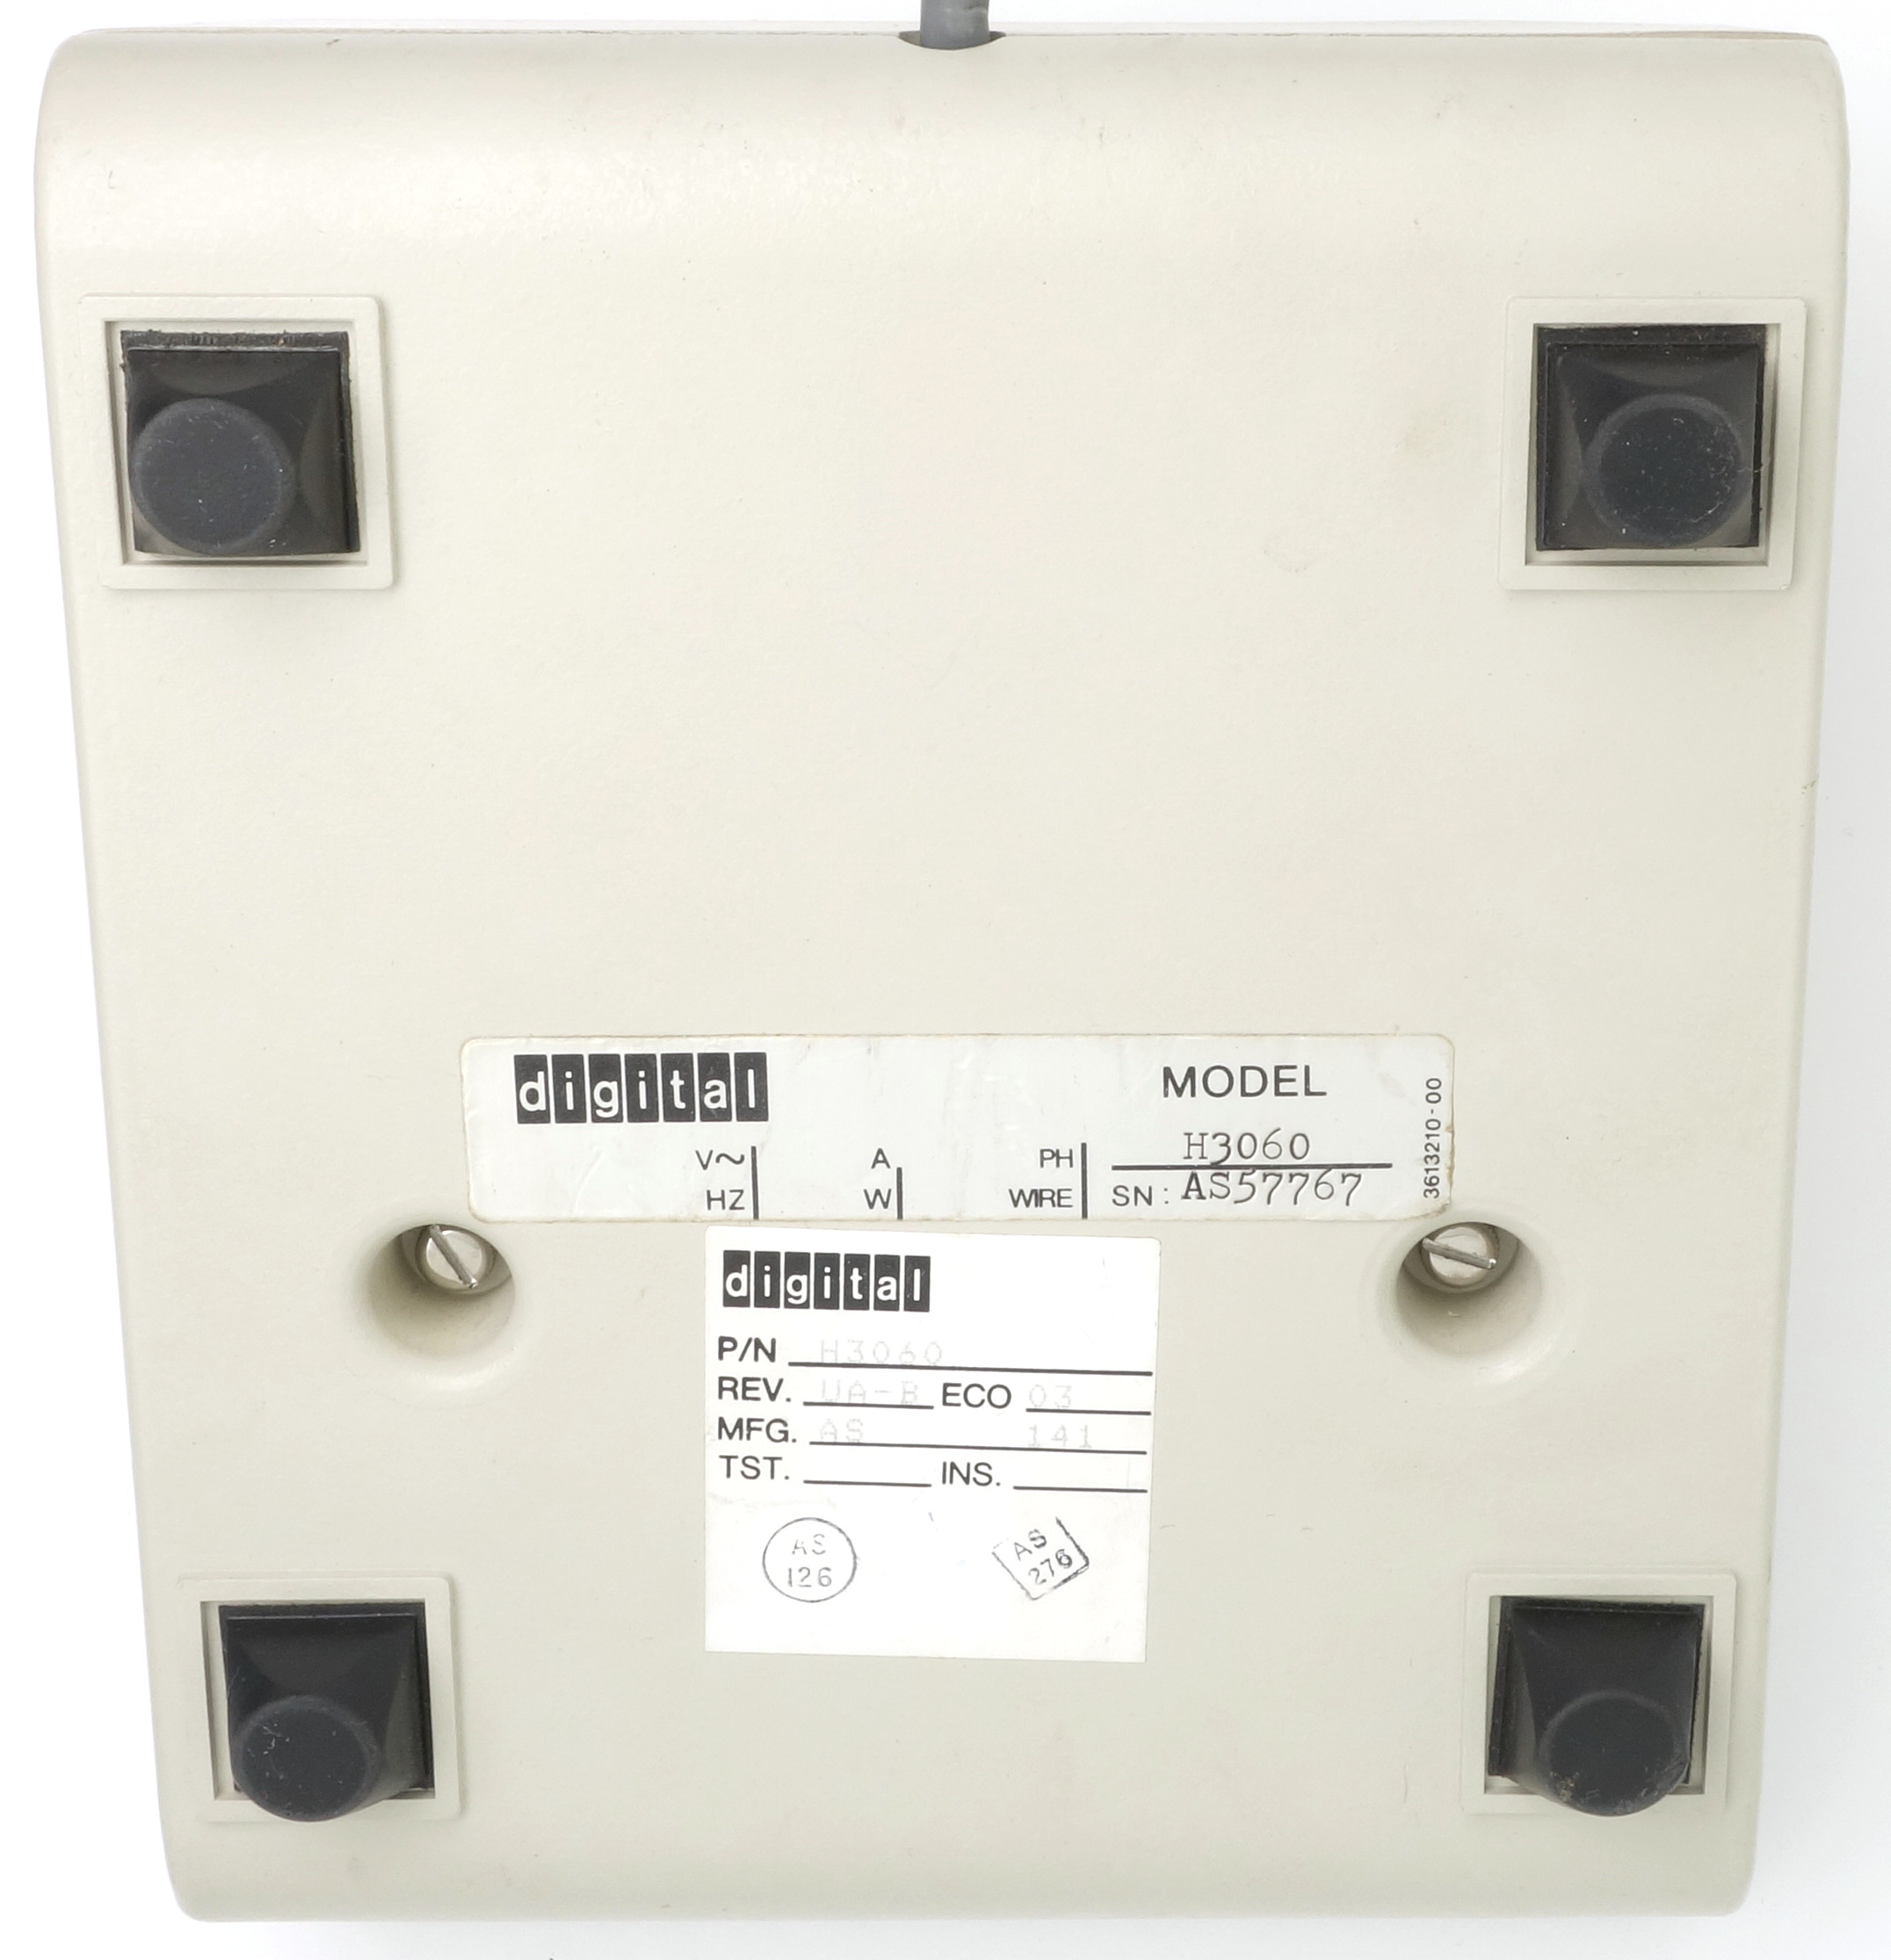
\includegraphics[scale=0.38]{1978_dec_h3060_joystick/bottom_15.jpg}
    \caption{Джойстик DEC H3060 joystick, вид сверху и снизу}
    \label{fig:DecJoystickTopAndBottom}
\end{figure}

Рукоятка джойстика является стандартным узлом: ее можно встретить в моделях других фирм, например в джойстике Tektronix 4952, выпущенном на рынок несколькими годами ранее. В отличие от рукоятки джойстика,  корпус устройства весьма крупный (рис. \ref{fig:DecJoystickSize}) - очевидно, из соображений эргономики и дизайна, а не для размещения электронных компонент.

Рукоятку джойстика достаточно удобно двигать, обхватив пальцами и опираясь кистью на корпус (рис. \ref{fig:DecJoystickHand}). Но <<переключатели прерываний>> --- это совсем другая история. Из-за своей конструкции они достаточно жесткие, не имеют четкого хода и не издают щелчок при нажатии. Поэтому при нажатии на них трудно дозировать усилие, и вопреки своему элегантному виду, они представляют собой одну из худших реализаций кнопок с точки зрения эргономики.

\begin{figure}[h]
    \centering
    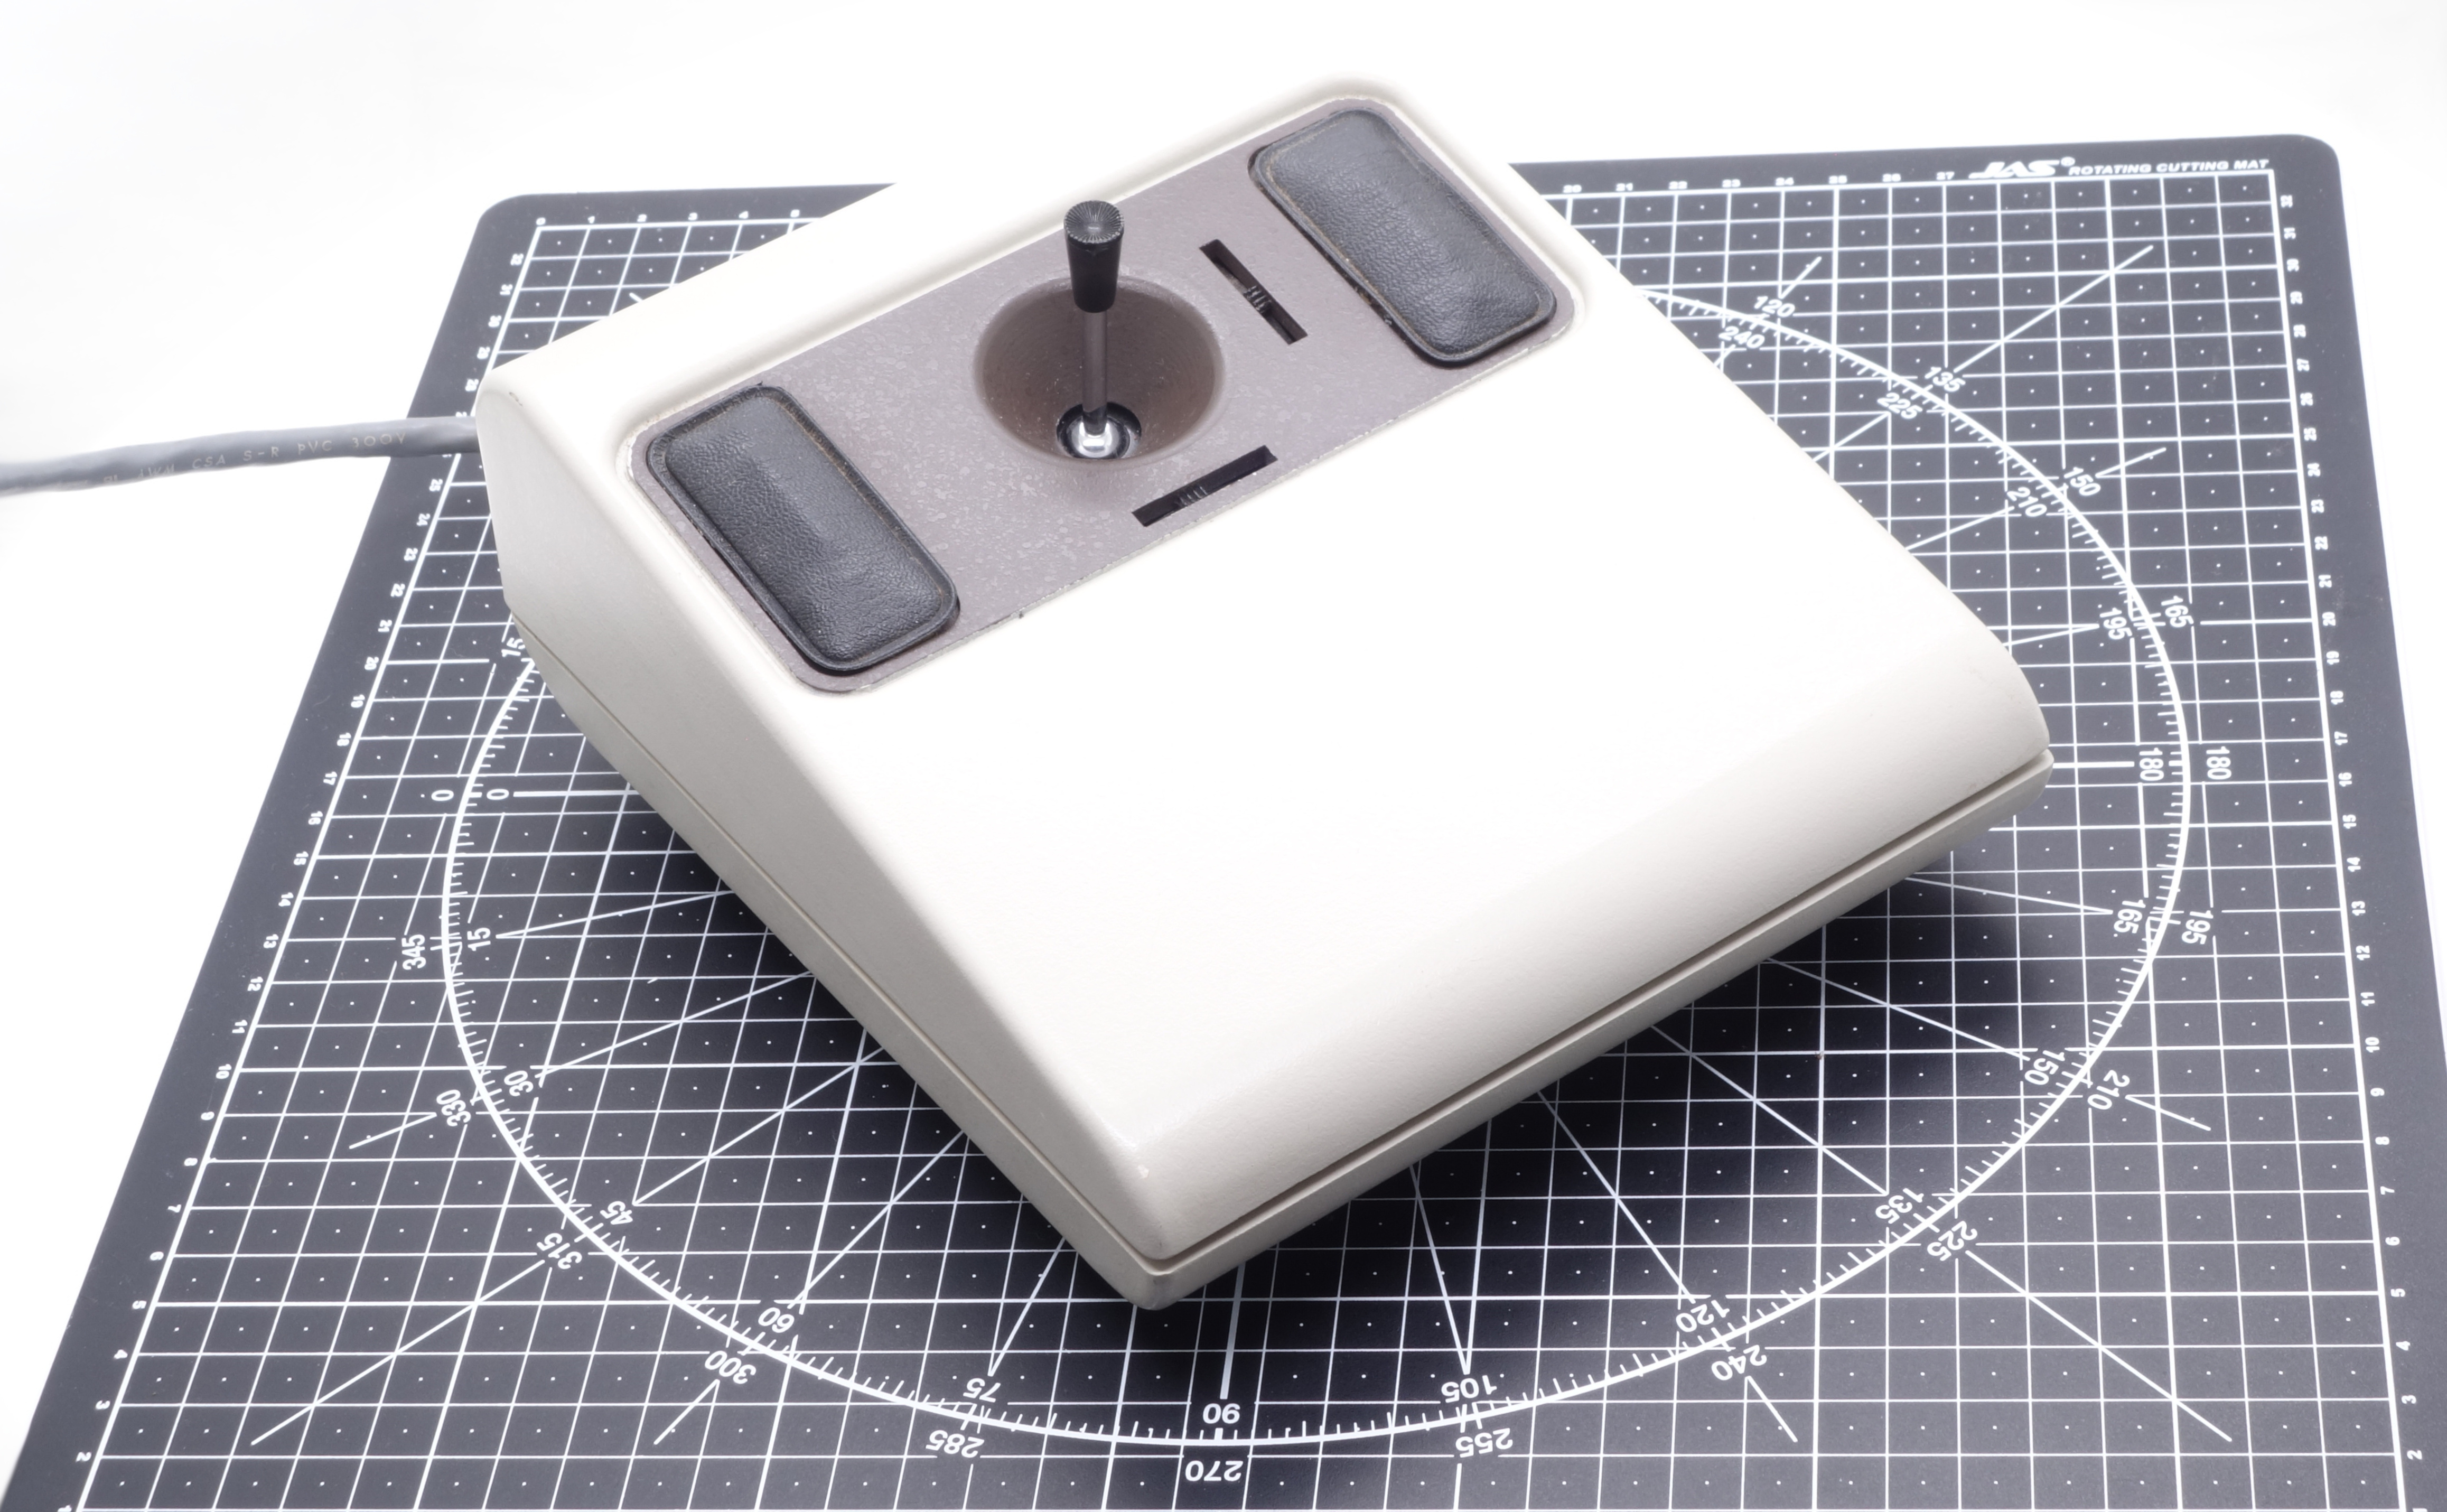
\includegraphics[scale=0.35]{1978_dec_h3060_joystick/size_30.jpg}
    \caption{Джойстик DEC H3060 на размерном коврике с шагом сетки 1~см}
    \label{fig:DecJoystickSize}
\end{figure}

Кнопки джойстика запараллелены и представляют собой один <<переключатель прерываний>>, генерирующий в зависимости от ситуации прерывание <<SWITCH>> (сигнал нажатия кнопки для отметки желаемой позиции на экране) либо прерывание <<CURSOR MATCH>> (выбор на экране объекта, контур которого пересекается с курсором). В последнем случае в момент прерывания дисплейный процессор прекращает выполнение «файла дисплея», оставляя текущий указатель позиции доступным для считывания выполняемой программой \cite{vsv11}. Этот подход изначально возник в системах с векторным дисплеем и световым пером, а затем был адаптирован для растровых дисплеев, таких как дисплей системы VS11/VSV11.

\begin{figure}[h]
    \centering
    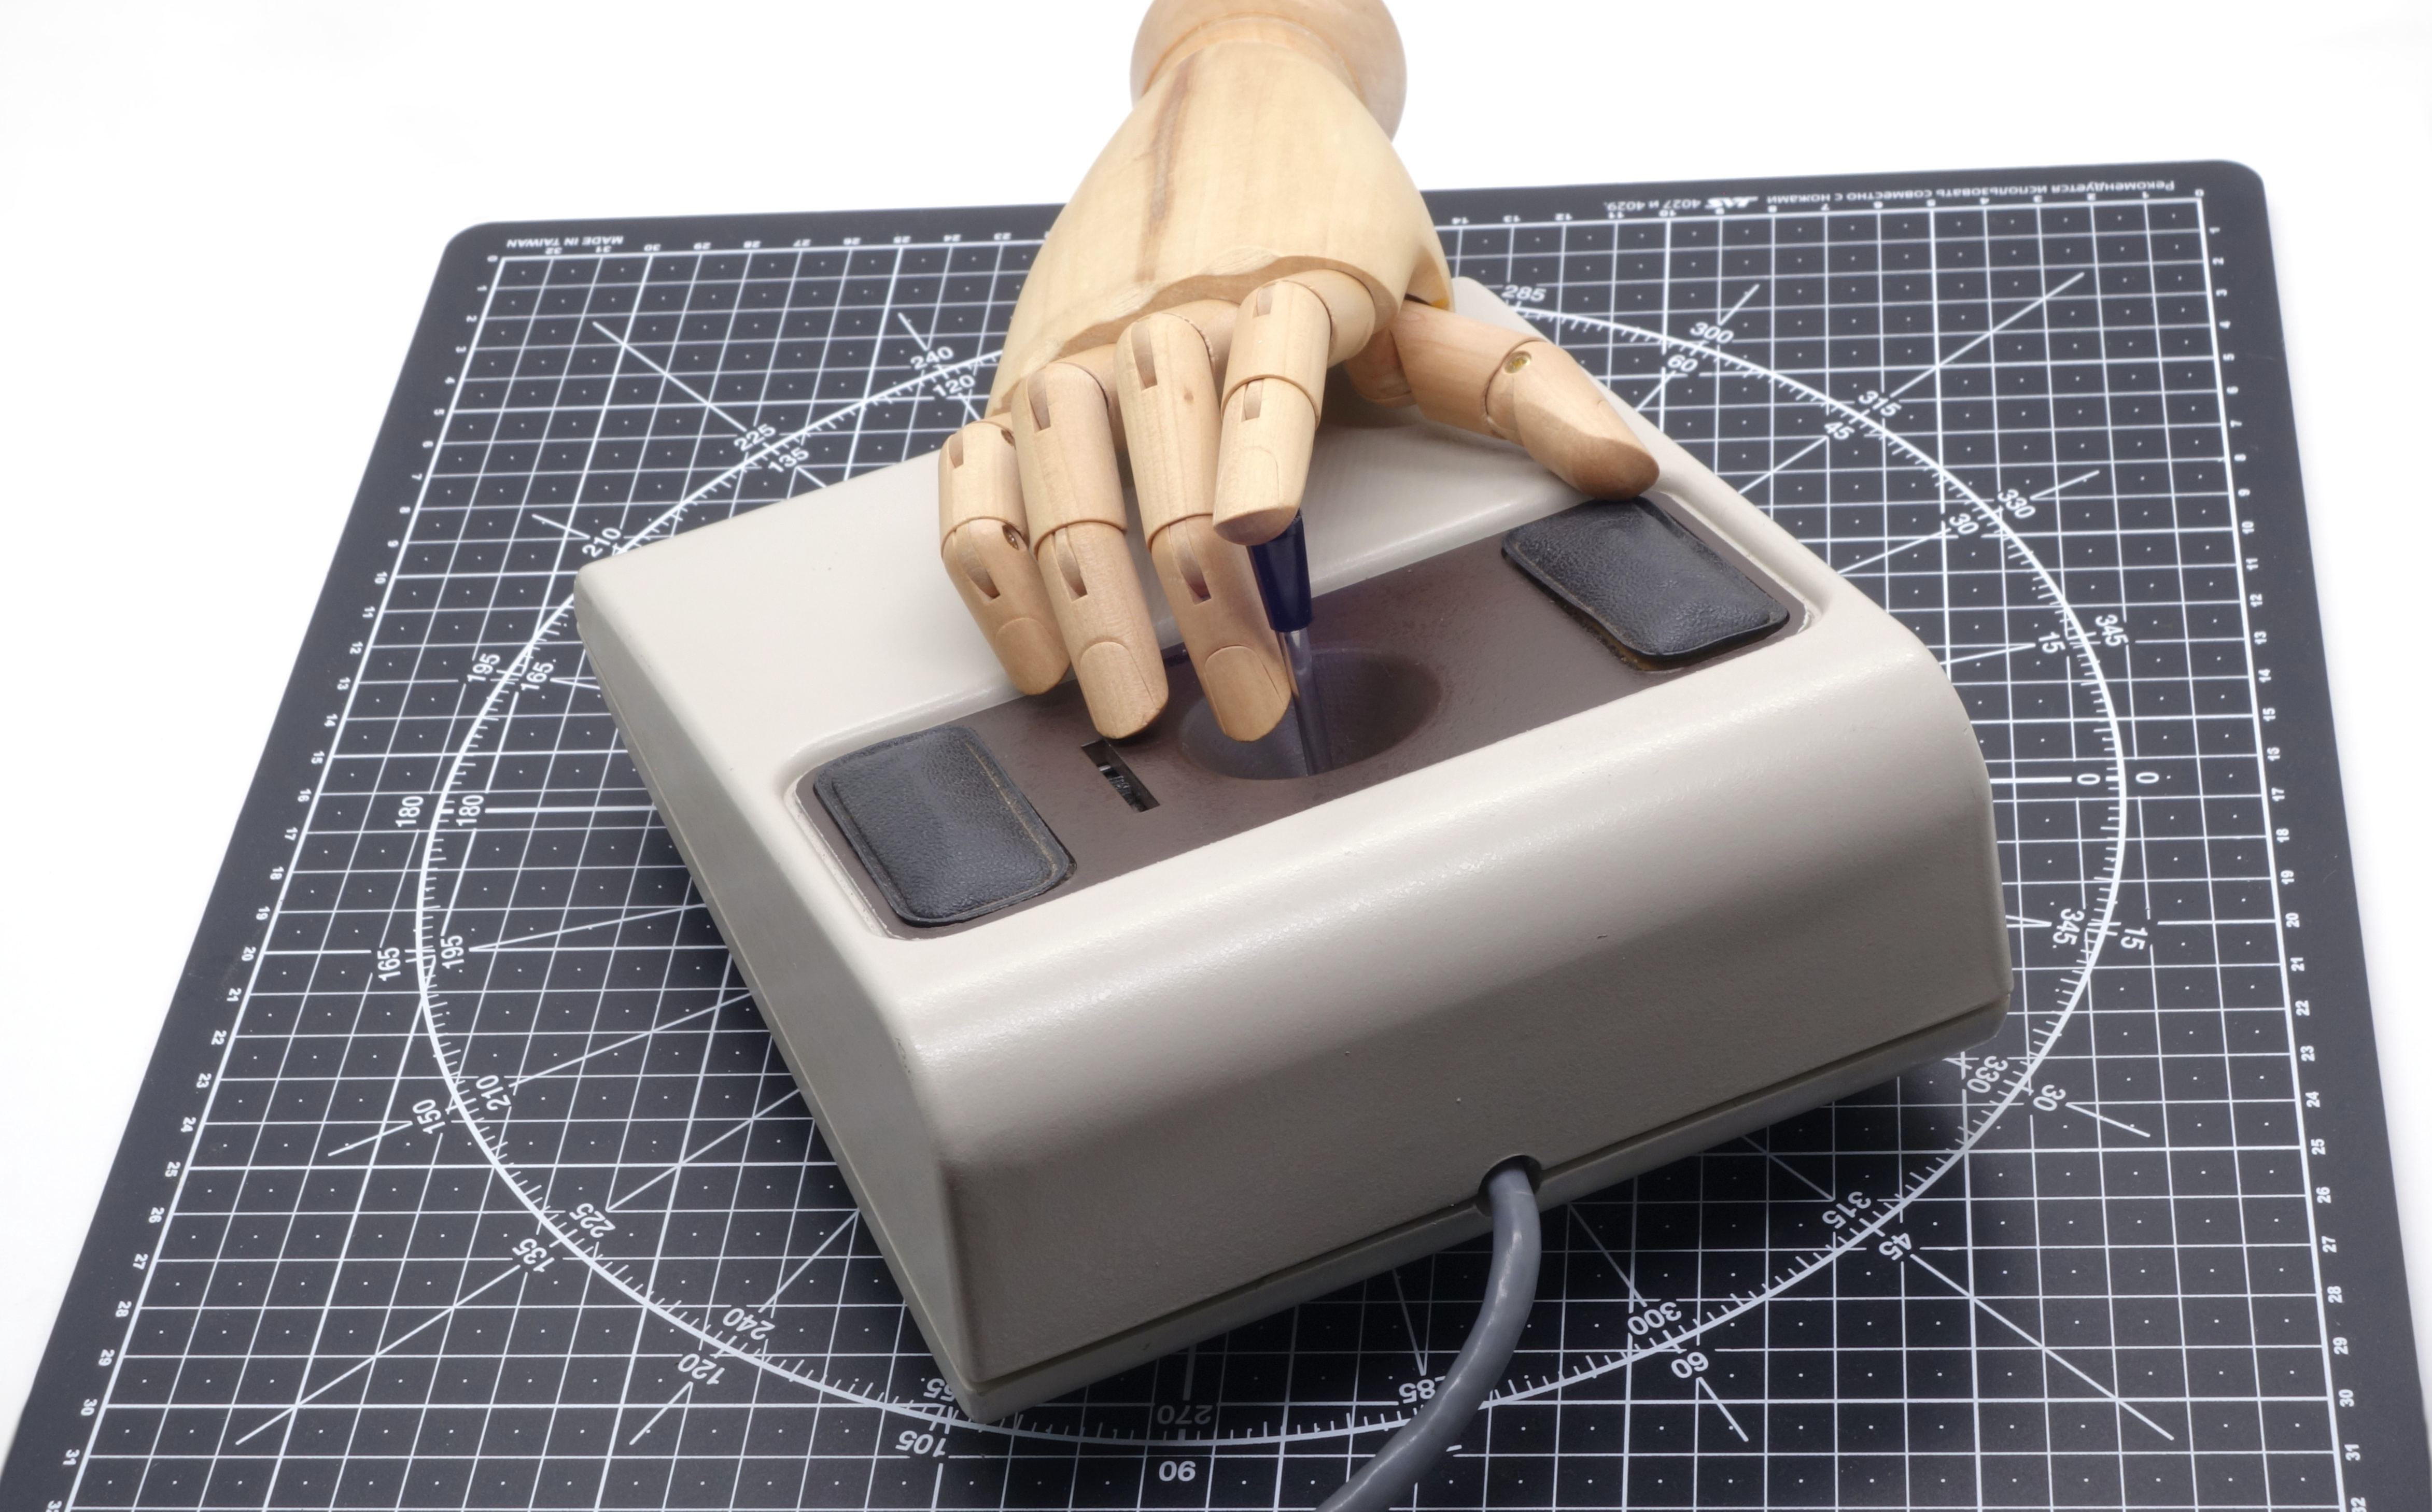
\includegraphics[scale=0.35]{1978_dec_h3060_joystick/hand_30.jpg}
    \caption{Джойстик DEC H3060 с моделью руки человека}
    \label{fig:DecJoystickHand}
\end{figure}

Наклон рукоятки влияет на движение курсора предсказуемым образом: направление движения определяется направлением наклона, а угол наклона пропорционален скорости движения. Триммеры используются для регулировки дрейфа путем выставления нулевого напряжения на выходах $X$ и $Y$ при вертикальном положении рукоятки.

При работе пользователь смещает курсор к нужной точке на дисплее, отклоняя рукоятку джойстика, но также курсор может перемещаться и программно путем записи в регистры координат дисплейного процессора.

Джойстик подключался к модулю VS11/VSV11 с помощью длинного толстого кабеля.


В разобранном виде джойстик показан на рис. \ref{fig:DecJoystickInside}. 

\begin{figure}[h]
    \centering
    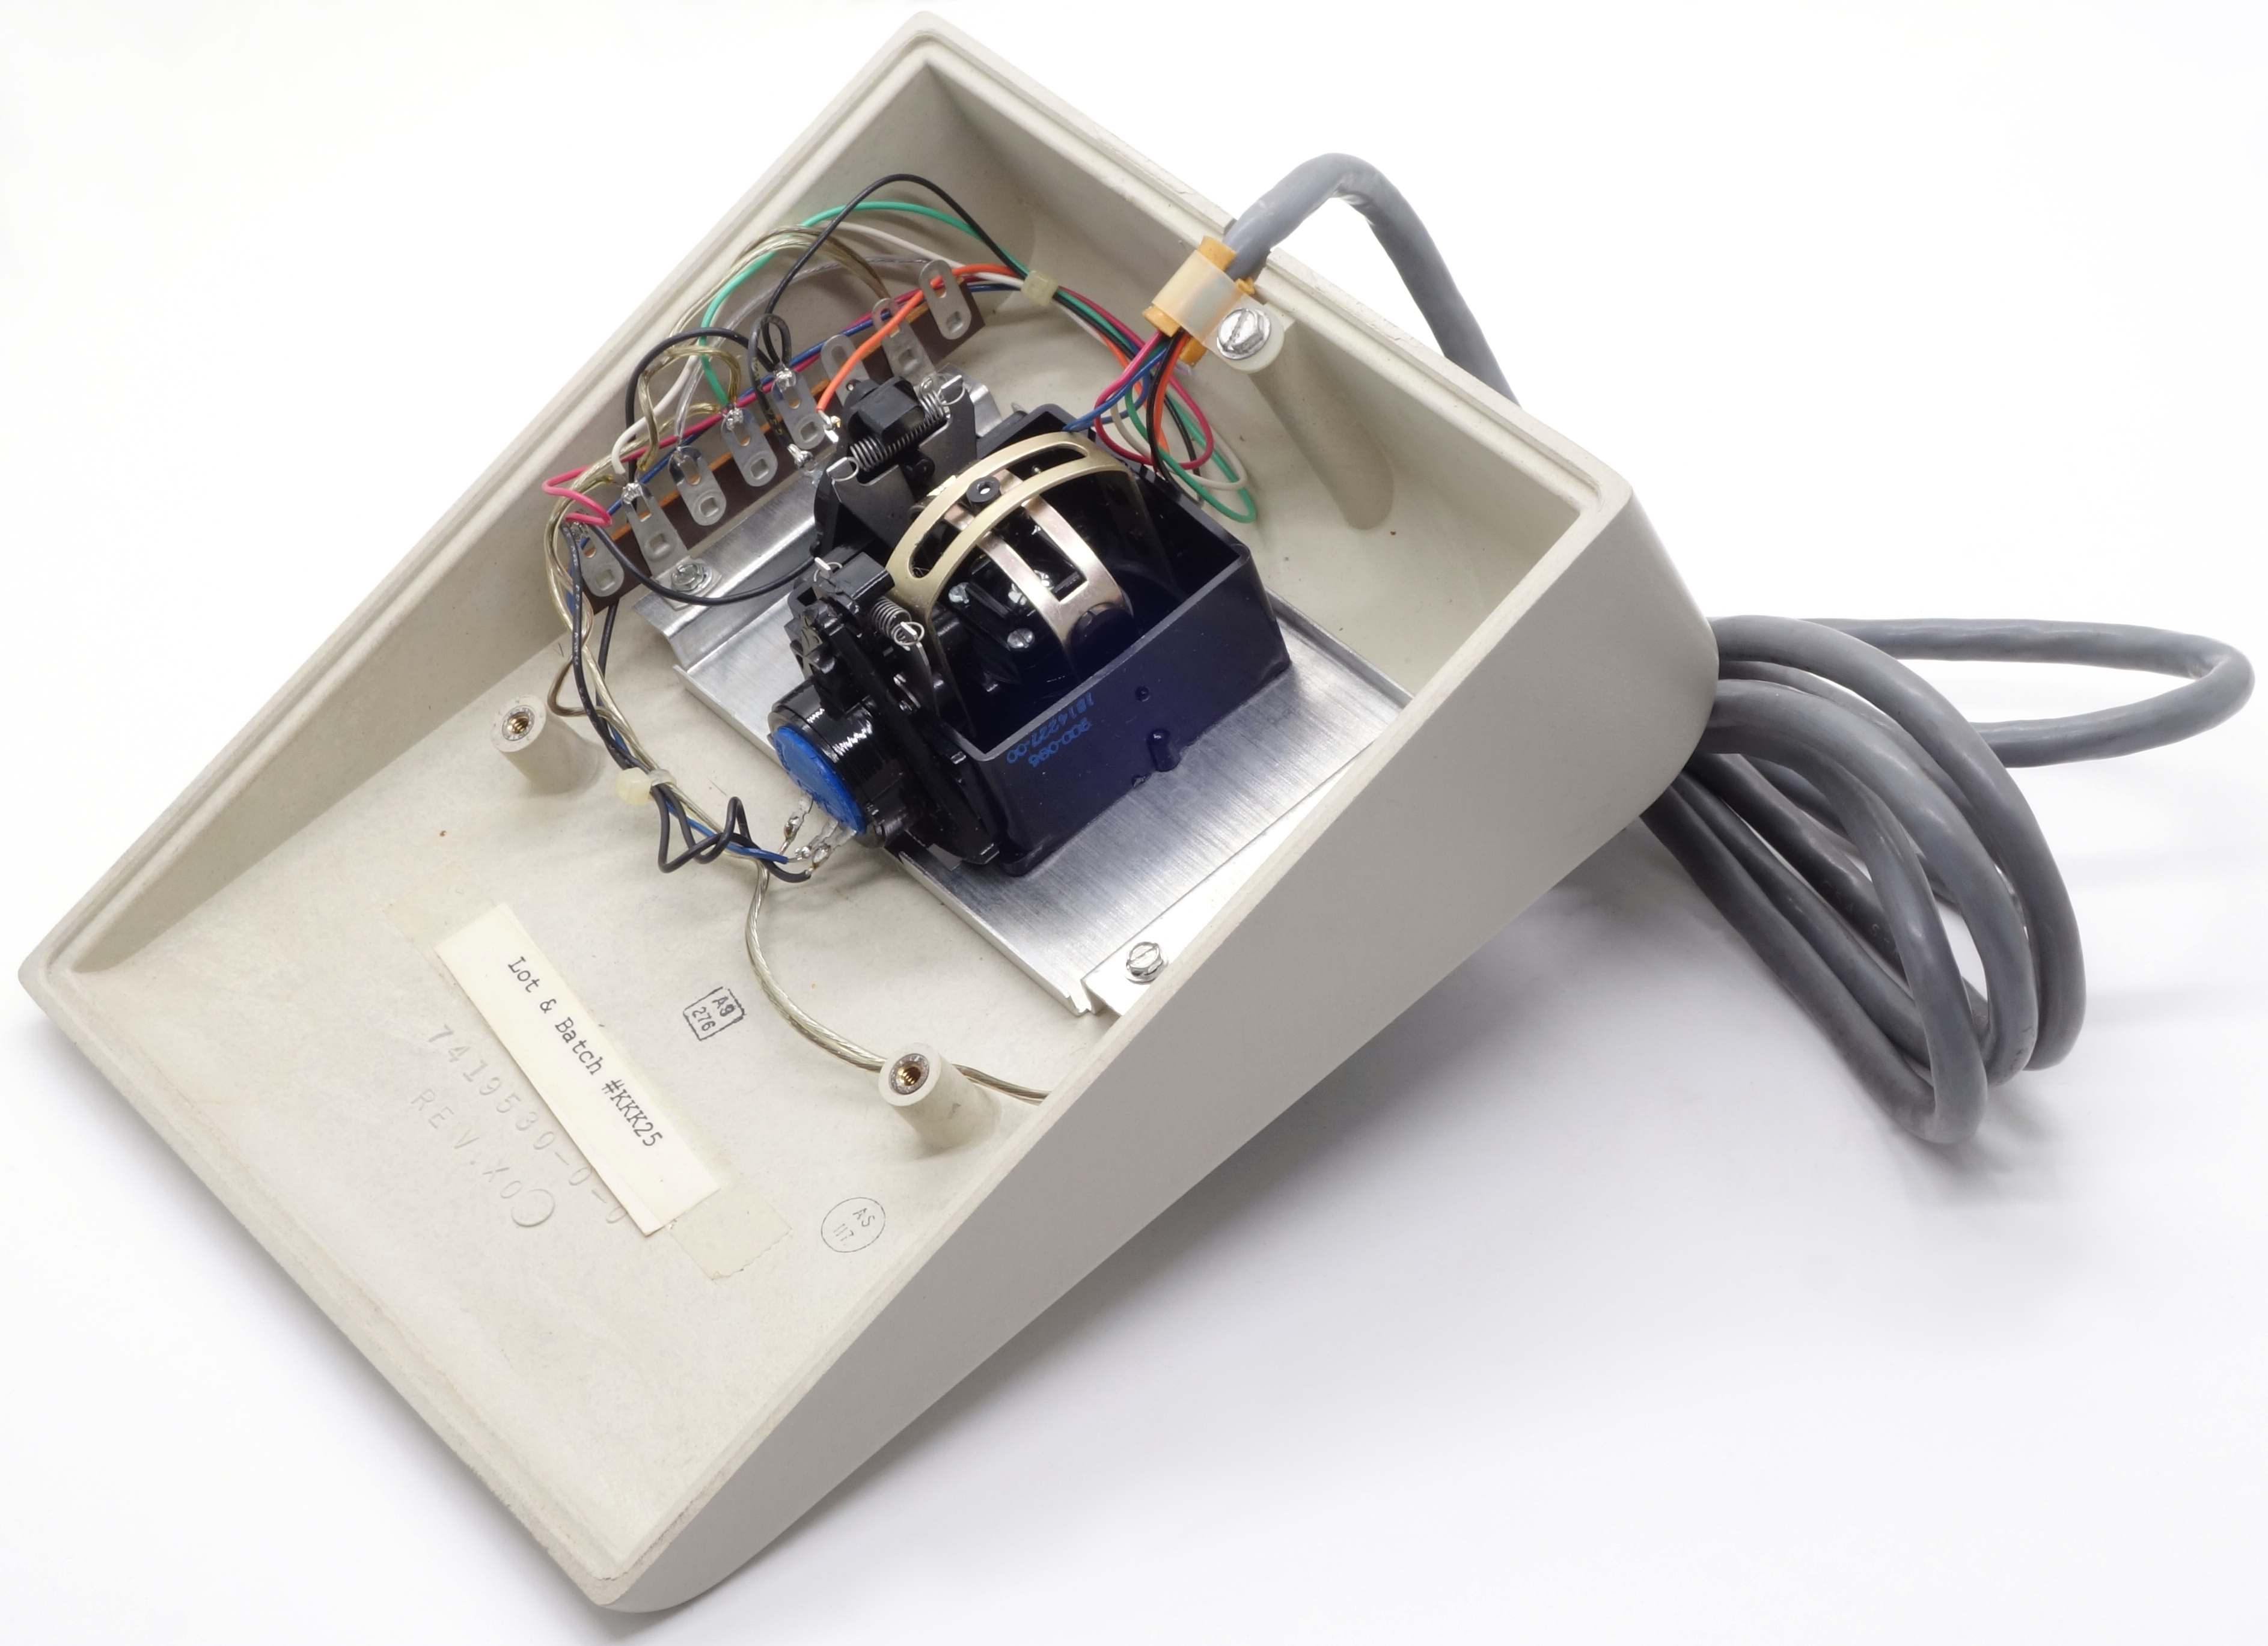
\includegraphics[scale=0.5]{1978_dec_h3060_joystick/inside_30.jpg}
    \caption{Джойстик DEC H3060 в разобранном виде}
    \label{fig:DecJoystickInside}
\end{figure}

Смещение триммеров обеспечивает контроль дрейфа путем механического поворота потенциометров $X$ и $Y$. 

Сборный узел джойстика, включая стержень рукоятки и его крепление, а также потенциометры и конструкцию поворотных узлов корректировки дрейфа, является типовым: в дальнейшем он встречается в неизменном виде, вплоть до полной взаимозаменяемости, во многих аналоговых джойстиках, выпускаемых для промышленных нужд.

\begin{thebibliography}{9}
\bibitem {joystick} VSV11 RASTER GRAPHICS SYSTEM. D\textbar I\textbar G\textbar I\textbar T\textbar A\textbar L CSS -- Computer Special Systems \url{https://www.pdp-11.nl/peripherals/comm/interface/vsv11/vsv11-info.html}
\bibitem {fiche} NCV-11 Diagnostic. DEC PDF-11 Diagnostic Program Listings. 1978. \url{bitsavers.informatik.uni-stuttgart.de/pdf/dec/pdp11/microfiche/Diagnostic_Program_Listings/Listings/CZNCCA0__NCV-11__DIAGNOSTIC__AH-E772A-MC__DEC_1978_bw.pdf}
\bibitem {flyer} VSV11 and VS11 Raster Graphics Systems. Digital Equipment Corporation. Jan 81 \url{https://ia804604.us.archive.org/17/items/TNM_VSV11_and_VS11_Raster_Graphics_Systems_-_digi_20171029_0045/TNM_VSV11_and_VS11_Raster_Graphics_Systems_-_digi_20171029_0045.pdf}
\bibitem{vsv11} VSV11/VS11 Raster Graphics System. Option Description. 1981. \url{https://archive.org/details/bitsavers_decgraphiconDescriptionDec81_14714530/mode/2up}
\end{thebibliography}
\end{document}
